\documentclass[twocolumn]{article}

%\usepackage[iso]{umlaute}
%\usepackage{german}
\usepackage{graphicx}
\usepackage{listings}
\usepackage{amsmath,amssymb,amsthm}
\usepackage{setspace}
\usepackage{hyperref}
\usepackage{mathpartir}
%\usepackage{courier}{
%\usepackage[left=1in,right=1in,top=1in,bottom=1in]{geometry}
\setlength{\parindent}{0cm}
\setlength{\columnsep}{25pt}
\sloppy
\setlength\parindent{24pt}
\newcommand{\lambdaLVar}{\ensuremath{\lambda_{\textrm{LVar}}}}
\newcommand{\lambdaLVish}{\ensuremath{\lambda_{\textrm{LVish}}}}
\newcommand{\userleq}{\ensuremath{\sqsubseteq}}
\newcommand{\Loc}{\mathit{Loc}}
\newcommand{\fmap}{\ensuremath{\stackrel{\textrm{fin}}{\rightarrow}}}
\newcommand{\setof}[1]{\left\{#1\right\}}
\newcommand{\topS}{\ensuremath{\top\hspace{-0.85mm}_{S}}}
\newcommand{\leqstore}[2]{\ensuremath{#1 \userleq_S #2}}
\newcommand{\LVarsDefStore}{
\begin{definition}[store, $\lambdaLVar$]\label{def:lvars-store}
A \emph{store} is either a finite partial mapping $S : \Loc \fmap (D
- \setof{\top})$, or the distinguished element $\topS$.
\end{definition}}
\newcommand{\dom}[1]{\ensuremath{\mathit{dom}(#1)}}
\newcommand{\userlub}[2]{\ensuremath{#1 \sqcup #2}}

%%% Metafunctions
\newcommand{\subst}[3]{\ensuremath{#1[#2 := #3]}}
\newcommand{\incomp}[1]{\ensuremath{\mathit{incomp}(#1)}}
\newcommand{\pred}[1]{\ensuremath{\mathit{pred}(#1)}}
\newcommand{\lubp}[2]{\ensuremath{#1 \sqcup_p #2}}
\newcommand{\qexist}[2]{\ensuremath{\exists\,#1.~#2}}
\newcommand{\qforall}[2]{\ensuremath{\forall\,#1.~#2}}
\newcommand{\userelements}{\ensuremath{\mathit{Elements}}}
\newcommand{\nuserleq}{\ensuremath{\not \sqsubseteq}}
\newcommand{\usergeq}{\ensuremath{\sqsupseteq}}
\newcommand{\userlt}{\ensuremath{\sqsubset}}
\newcommand{\leqp}{\ensuremath{\sqsubseteq_p}}
\newcommand{\ltp}{\ensuremath{\sqsubset_p}}
\newcommand{\botp}{\ensuremath{\bot_{p}}}
\newcommand{\topp}{\ensuremath{\top\hspace{-0.85mm}_{p}}}

%%% Stores and store operations
\newcommand{\StoreVal}{\ensuremath{\mathit{StoreVal}}}
\newcommand{\eqstore}[2]{\ensuremath{#1 =_S #2}}
\newcommand{\neqstore}[2]{\ensuremath{#1 \not =_S #2}}
\newcommand{\nleqstore}[2]{\ensuremath{#1 \not \userleq_S #2}}
\newcommand{\ltstore}[2]{\ensuremath{#1 \userlt_S #2}}
\newcommand{\lubstore}[2]{\ensuremath{#1 \sqcup_{S} #2}}
\newcommand{\glbstore}[2]{\ensuremath{#1 \sqcap_{S} #2}}
\newcommand{\storebindingRaw}[2]{\ensuremath{#1 \mapsto #2}}
\newcommand{\storebinding}[3]{\storebindingRaw{#1}{\state{#2}{#3}}}
\newcommand{\state}[2]{\ensuremath{(#1, #2)}}
\newcommand{\store}[1]{\left[ #1 \right]}
\newcommand{\extS}[4]{#1[\storebinding{#2}{#3}{#4}]}
\newcommand{\extSRaw}[3]{#1[\storebindingRaw{#2}{#3}]}
\newcommand{\storeset}{\mathcal{S}}
\newcommand{\status}{\ensuremath{\mathit{frz}}}
\newcommand{\frozentrue}{\ensuremath{\textsf{true}}}
\newcommand{\frozenfalse}{\ensuremath{\textsf{false}}}
\newcommand{\LVar}{\mathit{LVar}}

% Sans-serif font for terms of the language
\newcommand\termfont[1]{\mbox{\small{\texttt{#1}}}}
% Amount to indent the next line of a 'let' expression.
\newcommand{\letspace}{\hphantom{\termfont{le}}} % ``in'' should be under the ``t'' in ``let''
\newcommand{\letparspace}{\hphantom{\termfont{\LETPAR}}}
%%% Language forms.
\newcommand{\lam}[2]{\ensuremath{\lambda#1.\,#2}}
\newcommand{\app}[2]{\ensuremath{#1~#2}}
\newcommand{\unit}{\termfont{()}}
\newcommand{\NEW}{\termfont{new}}
\newcommand{\PUT}{\termfont{put}}
\newcommand{\PUTi}{\ensuremath{\termfont{put}_i}}
\newcommand{\putexp}[2]{\ensuremath{\PUT~#1~#2}}
\newcommand{\putiexp}[1]{\ensuremath{\PUT_i~#1}}
\newcommand{\GET}{\termfont{get}}
\newcommand{\getexp}[2]{\ensuremath{\GET~#1~#2}}
\newcommand{\UPDATE}{\termfont{update}}
\newcommand{\updateexp}[1]{\ensuremath{\update~#1}}
\newcommand{\GETFSTORSND}{\termfont{getFstOrSnd}}
\newcommand{\GETFST}{\termfont{getFst}}
\newcommand{\getfstexp}[1]{\ensuremath{\GETFST~#1}}
\newcommand{\GETSND}{\termfont{getSnd}}
\newcommand{\getsndexp}[1]{\ensuremath{\GETSND~#1}}
\newcommand{\FREEZE}{\termfont{freeze}}
\newcommand{\AFTER}{~{\termfont{after}}}
\newcommand{\WITH}{~{\termfont{with}}}
\newcommand{\ADDHANDLER}{{\termfont{addHandler}}}
\newcommand{\NEWPOOL}{{\termfont{newPool}}}
\newcommand{\ADDHANDLERINPOOL}{{\termfont{addInPool}}}
\newcommand{\QUIESCE}{{\termfont{quiesce}}}
\newcommand{\FAW}{{\termfont{freeze}-\termfont{after}-\termfont{with}}}
\newcommand{\freeze}[1]{\ensuremath{\FREEZE~#1}}
\newcommand{\freezeafter}[3]{\ensuremath{\FREEZE~#1~\AFTER~#2~\WITH~#3}}
\newcommand{\freezeafterfull}[5]{\ensuremath{\FREEZE~#1~\AFTER~#2~\WITH~#3, #4, #5}}
\newcommand{\LET}{\termfont{let}}
\newcommand{\PAR}{\termfont{par}}
\newcommand{\LETPAR}{\termfont{\LET~\PAR}}
\newcommand{\IN}{\termfont{in}}
\newcommand{\letexp}[3]{\ensuremath{\LET~#1=#2~\IN~#3}}
\newcommand{\letparexp}[5]{\ensuremath{\LETPAR~#1=#2;~#3=#4~\IN~#5}}
\newcommand{\stateset}[1]{\ensuremath{\lbrace #1 \rbrace}}

% Your name
\author{Nishanth Nagendra \\ Technische Universit\"at M\"unchen}

\title{Seminar: Programming models and Code Generation\\
       Winter Term 2014/2015\\
       {\bf Quasi deterministic parallel programming using LVars}
}

% Date of your talk
\date{15.01.2015}


\begin{document}

\maketitle

\begin{abstract}
A \textit{deterministic program} always produces the same observable result on multiple runs. A \textit{deterministic by construction parallel programming model} allows only such programs to be written offering programmers freedom from hard to reproduce non deterministic bugs. This report talks about \textit{Lvish}, a \textit{quasi deterministic parallel programming model} that extends \textit{LVars}, its predecessor, which is a \textit{deterministic model}. LVars generalize existing single assignment models by allowing communication through shared monotonic data structures with monotonic write operations and threshold read operations that block until a lower bound is reached. The semantics are defined in terms of an application specified lattice. LVish extends LVar by allowing to freeze them in order to read their exact contents and to attach event handlers to an LVar triggering a callback when their state changes. It offers quasi determinism in the worst case which means on every run it either produces the same result or raises an error. The LVish model yields promising parallel speedup on benchmarking applications using a prototype implementation of a library in haskell.
\end{abstract}

% \section defines numbered parts of the paper with titles
% there also are \subsection and \subsubsection
\section{Introduction}

% Use labels to be able to refer to this position from somewhere else
\label{introduction}

The purpose of a deterministic-by-construction programming model is to rule out programs like the following from being written, or force them to behave deterministically. Written in a hypothetical parallel language~\cite{lindsey}. "\texttt{\_}" below refers to an anonymous variable.
\begin{verbatim}
let _ = put lv 3 in  /write 3 in lv/
let par v = get lv  /read from lv/
        _ = put lv 4  /write 4 in lv/
	      in v   /final value is v/
\end{verbatim} 
The \textit{let par} expression which has \textit{fork-join semantics}, evaluates the two sub-expressions in parallel. The value of $v$ is the value of the entire program. Depending on the scheduler \textit{get} $lv$ or \textit{put} $lv\ 4$ can run first, $v$ might be either $3$ or $4$ during multiple runs giving rise to non determinism.\par
A popular approach for enforcing determinism is to require that variables can only be assigned to once, giving us a single-assignment language so the above program would be invalid because it tries to write to $lv$ twice. Single-assignment variables with blocking read semantics, often known as IVars, turn up in all kinds of deterministic parallel systems. But the single-assignment rule disallows a number of programs that we would like to permit such as writing the same value to an IVar twice. As another example, consider the problem of filling in various parts of a data structure in parallel. \cite{lindsey}Say that $lv$ contains a pair, and we are writing to $lv$ twice, with each write filling in one component of the pair. 
\begin{verbatim}
let par  _ = put lv (4,x)
         _ = put lv (x,3) /error/
         in get lv
\end{verbatim}  
Please note that $x=\bot$ above. Read from $lv$ is possible once both writes have completed, so it will always be (4, 3). But single-assignment rules out this program(although we could fake it by using a distinct IVar for each component of the pair, but with more sophisticated data structures it becomes difficult to fake a solution with IVars.)\par

There is a need to generalize the single-assignment model to admits programs like these but retain determinism. Deterministic algorithms must be expressible in a style that guarantees determinism, and non-deterministic behaviors, where desired, must be requested explicitly. Enforcing deterministic semantics simplifies composing, porting, reasoning about, debugging, and testing parallel software. Existing models tend to lack features and extensibility that would make them applicable to a broader range of problems.\\ \\
\textit{\textbf{Existing models}}\cite{kuper} A number of models currently exist as a part of the long running effort towards deterministic by construction parallel programming. \par
\begin{itemize}
        \item \textit{No-shared-state parallelism}: Pure functional programming in Haskell with par and pseq combinators is an example. It uses function level task parallelism or futures. This kind of parallelism does not allow for any shared mutable state between tasks, forcing tasks to produce values independently. Models based on pure data parallelism like \textit{Data parallel Haskell, River Trail API for Java script} also fall in this category,
        \item \textit{Data-flow parallelism}: Kahn process networks, snychronous data flow systems are examples. In these models, tasks can only communicate via channels which are FIFO queues where the read operation on these queues is blocking until data is available. Stream-processing languages such as \textit{StreamIt} are based on KPN. 
        \item \textit{Single-assignment parallelism}: IVars are an example which are memory locations that can be either full or empty and can only be assigned once. Reads are blocking for IVars. They have been used in the \textit{monad-par} Haskell library, \textit{Intel CnC(Concurrent collections), Concurrent ML(as SnycVars)}.
        \item \textit{Imperative-disjoint parallelism}: The state accessed by concurrent threads are disjoint. \textit{Deterministic Parallel Java} falls under this category.     
\end{itemize} 
A common theme that emerges in the study of \textit{deterministic-by-construction systems} is the notion of monotonicity. Many deterministic parallel programs cannot be expressed with these models. Sharply restricted communication and synchronization capabilities have consequences not only for the immediate usability of guaranteed-deterministic languages, but for the extensibility of those languages as well.
\\ \\ 
\textit{\textbf{Motivating Example}} Consider applications in which independent sub-computations contribute information to shared data structures that are unordered, irregular, or application-specific. Following is an example that highlights the issues of ordering which create a friction between parallelism and determinism. \par 
In a directed graph where v represents a particular node, we wish to find all (or the first k degrees of) node connected to v, then analyze each node in that set. Existing parallel solutions\cite{kuper} often use a non-deterministic traversal of the connected component even though the final connected component is deterministic and IVars and Streams are not of much help. For example, IVars cannot accumulate sets of visited nodes, nor can they be used as “mark bits” on visited nodes, since they can only be written once and not tested for emptiness. Streams, on the other hand, impose an excessively strict ordering for computing the unordered set of vertex labels in a connected component. A purely functional attempt is given in the original paper\cite{lkuper} where connected-component discovery is parallel, but members of the output set do not become available to other computations until component discovery is finished, limiting parallelism. 
An LVars\cite{lkuper} based programming model can possibly allow us to write a breadth first search traversal where threads communicate using shared monotonic data structures. Consumers of the data structure may execute as soon as data is available, but may only observe irrevocable, monotonic properties of it. 

\section{LVars and LVish}
\subsection{LVars}
An LVar is a memory location that can be shared between multiple threads whose contents can only grow bigger over time, for some definition of “bigger” that the user of the LVar gets to specify. \par
LVars, short for lattice variables, are a generalization of IVars, which are variables that can only be written to once. (The “I” is for “immutable”.) LVars, on the other hand, allow multiple writes, as long as those writes are monotonically increasing with respect to a user-specified lattice. Meanwhile, LVar reads have to specify a threshold set of possible states. A read will block until one of the states in the threshold set has been reached, and then return that state. Information can never be removed and the order in which it is added is not observable. IVars turn out to be a special case of LVars. 
The property of monotonically increasing write operations is enforced by the language. The semantics of $put$ says that the write to a location is the least upper bound of the new value and the current value. 
\begin{verbatim}
let par _ = put num 3
        _ = put num 2
        x = get num
  in x  /*could be 2 or 3*/
\end{verbatim}
Monotonic writes alone aren't enough to ensure determinism. The above program is non-deterministic where num's notion of “bigger” is $\geq$. Despite writes always being monotonically increasing. $Get$ might read either $2$ or $3$, depending on the order of $put$ or $get$ operations determined by the scheduler. With an LVar model this behavior changes.\par
\begin{itemize}
\item To maintain determinism, the LVars model restricts the $get$ operation. Instead of reading the LVar’s exact value, it reads one of a set\{threshold set\} of lower bounds on its value that are given as an extra argument to $get$ not shown in the example. The $get$ operation will block until the LVar reaches a value that is at or above one of those lower bounds. For the above example, the threshold set will just be \{$3$\}. $get$ operation is called a threshold read, because the value it returns is the threshold we have crossed.
\item Once num value is atleast $3$, it will remain at or above $3$ forever. As long as we only access them through the $put$ or $get$ interface, LVars are thread-safe: we can safely share them between threads without introducing unintentional non-determinism. That is, $puts$ and $gets$ can happen in any order, without changing the value that a program evaluates to.
\end{itemize}
%\begin{center}
%\textit{Monotonically increasing writes + threshold reads = deterministic parallelism}
%\end{center}
The resulting model is general enough to subsume the existing single-assignment model. The user-specified set just needs to be a \textit{join-semilattice}, which is a partially ordered set in which every two elements have a least upper bound. 

To describe Lvar formally, a parallel call-by-value $\lambda$-calculus named $\lambdaLVar$ is introduced in \cite{lkuper} which is extended with a $store$ and communication primitives $put$ and $get$ that operate on data in the $store$. The definition of $\lambdaLVar$ is parameterized by the choice of lattice and therefore $\lambdaLVar$ is actually a family of languages, rather than a single language. An LVar may have an arbitrary number of states forming a set $D$, which is partially ordered by a relation $\userleq$. Formally, $D$ is a \emph{bounded-join-semilattice} augmented with a greatest element $\top$. 
\begin{itemize}
\item $D$ has a least element $\bot$, representing the initial “empty” state of an Lvar,
\item $D$ has a greatest element $\top$, representing the “error” state that results from conflicting updates to an Lvar,
\item $D$ comes equipped with a partial order $\userleq$, where $\bot \userleq d \userleq \top$ for all $d \in D$.
\item Every pair of elements in $D$ has a least upper bound (lub) written $\sqcup$ which means it is possible for two sub-computations to independently update an LVar, and then deterministically merge the results by taking the lub of the resulting two states.
\end{itemize}
% free floating figure using width of full page, to be put on [t]op.
\begin{figure}
\centerline{
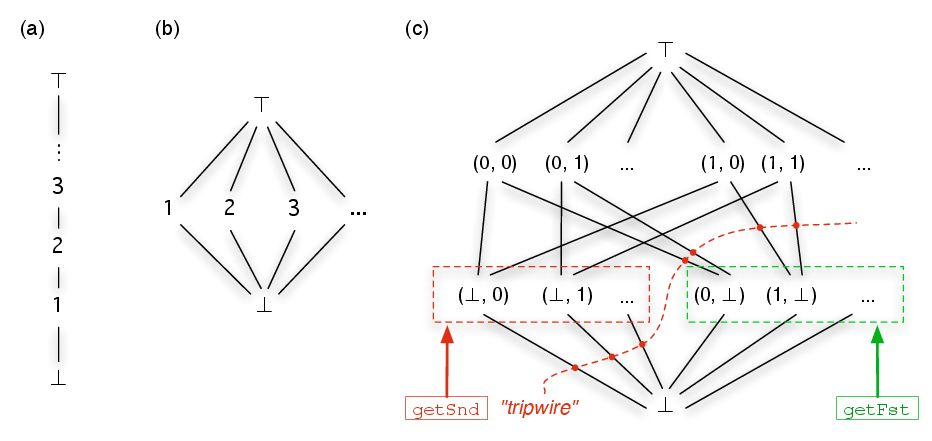
\includegraphics[width=1.0\columnwidth]{Figures/lattice.jpg}
}
\caption{Example lattices\cite{lkuper}: (a) Positive integers ordered by $\leq$ (b) IVar containing a natural number (c) Pair of natural number-valued IVars}
\label{Figure1}
\end{figure}
Data structures like arrays, tree, maps , streams etc. can be represented  as lattice. $Figure$ $2$ gives three examples of lattices for common data structures.
 
During the evaluation of a $\lambdaLVar$ program, a \emph{store} $S$ keeps track of the states of LVars. Each LVar is represented by a \emph{binding} from a location \emph{$l$}, drawn from a countable set $\Loc$, to its \emph{state}, which is some element $d \in D$. Although each LVar in a program has its own state, the states of all the LVars are drawn from the same lattice $D$. We can do this with no loss of generality because lattices corresponding to different types of LVars could always be union-ed into a single lattice (with shared $\bot$ and $\top$ Elements). \\ \\
\textbf{Definition 1}: A \emph{store} is either a finite partial mapping $S : \Loc \fmap (D - \setof{\top})$, or the distinguished element $\topS$. \\ \\
The state space of $stores$ forms a \emph{bounded-join-semilattice} augmented with a greatest element, just as $D$ does, with the empty store $\bot_S$ as its least element and $\top_S$ as its greatest element. The $\userleq$ and $\sqcup$ operations defined on elements of $D$ can be lifted to the level of stores.\\ \\
\textbf{Definition 2}: 
 A store $S$ is \emph{less than or equal to} a store $S'$ (written
$\leqstore{S}{S'}$) iff:
\begin{itemize}
\item $S' = \topS$, or
\item $\dom{S} \subseteq \dom{S'}$ and for all $l
\in \dom{S}$, $S(l) \userleq S'(l)$.
\end{itemize}
\textbf{Definition 3}:  The lub of stores $S_1$ and $S_2$ (written $\lubstore{S_1}{S_2}$) is
defined as follows:
\begin{itemize}
\item $\lubstore{S_1}{S_2} = \topS$ iff there exists some $l \in
\dom{S_1} \cap \dom{S_2}$ such that $\userlub{S_1(l)}{S_2(l)} = \top$.
\item Otherwise, $\lubstore{S_1}{S_2}$ is the store $S$ such that:
\begin{itemize}
\item $\dom{S} = \dom{S_1} \cup \dom{S_2}$, and
\item For all $l \in \dom{S}$:
\end{itemize}
\begin{displaymath}
S(l) = \left\{ \begin{array}{ll}
\userlub{S_1(l)}{S_2(l)} & \textrm{if $l \in \dom{S_1} \cap \dom{S_2}$} \\
S_1(l) & \textrm{if $l \notin \dom{S_2}$} \\
S_2(l) & \textrm{if $l \notin \dom{S_1}$}
\end{array} \right.
\end{displaymath}
\end{itemize}
\textbf{\textit{By Definition 3:}}, if $\userlub{d_1}{d_2} = \top$, then $\lubstore{\store{\storebindingRaw{l}{d_1}}}{\store{\storebindingRaw{l}{d_2}}} = \topS$. Notice that a store containing a binding $\storebindingRaw{l}{\top}$ can never arise during the execution of a $\lambdaLVar$ program, because an attempted write that would take the state of $l$ to $\top$ would raise an error before the write can occur.\\ \\
\textbf{\textit{Communication Primitives}}
The $new$, $put$, and $get$ operations create, write to, and read from LVars, respectively.
\begin{itemize} 
\item $new$ extends the $store$ with binding for a new LVar whose initial state is $\bot$, and returns the location $l$ of that LVar (a pointer to the LVar).
\item $put$ takes a pointer to an LVar and a singleton set containing a new state and updates the LVar’s state to the least upper bound of the current state and the new state, potentially pushing the state of the LVar upward in the lattice. Any update that would take the state of an LVar to $\top$ results in an error.\\
\item $get$ performs a blocking “threshold” read. It takes a pointer to an Lvar and a \emph{threshold set} $Q$, which is a non-empty subset of $D$ that is \emph{pairwise incompatible}, meaning that the lub of any two distinct elements in $Q$ is $\top$. If the LVar's state $d_1$ in the lattice is \emph{at or above} some $d_2 \in Q$, the $get$ operation unblocks and returns $d_2$. Note that $d_2$ is a unique element of $Q$, for if there is another $d_2' \neq d_2$ in the threshold set such that $d_2' \userleq d_1$, it would follow that $d_2 \sqcup d_2' \userleq d_1$, which contradicts the requirement that $Q$ be pairwise incompatible.
\end{itemize}
\begin{figure}
\begin{mathpar}
\inferrule*
{\lbrace p \rbrace ~ C ~ \lbrace q \rbrace}
{\lbrace p * r \rbrace ~ C ~ \lbrace q * r \rbrace}
\end{mathpar}
\caption{Standard frame rule.}
\label{f:frame-rule}
\end{figure}
For $\lambdaLVar$ syntax and semantics, remaining definitions and its details please refer\cite{lkuper}.\\ \\ 
\textbf{\textit{Proof of determinism:}} The key to the determinism is the frame rule given in \ref{f:frame-rule}. A frame property captures the idea of local reasoning about programs that alter state\cite{lindsey}. Here, $C$ is a program, and $\{p\} C \{q\}$ says that if the assertion $p$ is true before $C$ runs, then the assertion $q$ will be true afterwards. For example, $p$ and $q$  might describe the state of the heap before and after it is updated by $C$. It tells that running $C$ starting from a state satisfying the assertion $p$ $\ast$ $r$ will result in a state satisfying the assertion $q$ $\ast$ $r$. The assertion $p$ $\ast$ $r$ is satisfied by a heap if the heap can be split into two non-overlapping parts satisfying $p$ and $r$, respectively.

For LVars, the frame property says that independent effects commute with each other. Consider an expression $e$ that runs starting in \emph{store S} and steps to the expression $e^{'}$, updating the \emph{store} to $S^{'}$. Frame property guarantees that if $e$ starts from a larger $store\ S$ $\sqcup$ $R$, where $R$ is some other $store$ \emph{“framing on”} to $S$, then $e$  will update the $store$ to $S^{′}$ $\sqcup$ $R$, and $e$ will step to $e^{′}$. The \emph{“frame”} \emph{store} $R$  is a \emph{store} resulting from some other independently-running computation. $S$ and $R$ (or $S^{′}$ and $R$) need not be disjoint, we are combining them with $\sqcup$, not with $\ast$. If they did have to be disjoint, it would mean that concurrent operations cannot touch the same parts of the store. For LVars, this kind of total disjointness is unnecessary, since updates commute! Instead, we can behave as though $S$ and $R$ are disjoint, even though they might not be. \\ \\
\textbf{\textit{Diamond Lemma:}} This does the heavy lifting of the determinism proof: it establishes the diamond property, which says that if a configuration steps to two different configurations, there exists a single third configuration to which those configurations both step. For supporting lemmas, its details and complete proofs please refer to\cite{lkuper}. Lemmas there also show how cases of deadlocks and livelocks are also handled.

The LVars model guarantees determinism by monotonic write operations[which can commute] and threshold read operations. But it is not as general-purpose as one might hope. Consider an unordered graph traversal. A typical implementation involves a monotonically growing set of \emph{“seen nodes”}; neighbors of seen nodes are fed back into the set until it reaches a fixed point. These are not expressible using the threshold read and least-upper-bound write operations described above. The problem is that these computations rely on negative information about a monotonic data structure, i.e., on the absence of certain writes to the data structure. In a graph traversal, neighboring nodes should only be explored if the current node is not yet in the set; a fixpoint is reached only if no new neighbors are found; and at the end of the computation it must be possible to learn exactly which nodes were reachable. But in the LVars model, asking whether a node is in a set means waiting until the node is in the set, and it is not clear how to lift this restriction while retaining determinism.
\subsection{LVish}
Lvish\cite{lkuper2} extends the Lvars model with 2 additional capabilities. First, it adds event handlers, a mechanism for attaching a callback function to an LVar that runs, asynchronously, whenever events arrive (in the form of monotonic updates to the Lvar). Second, a primitive for freezing an LVar, which means: once an LVar is frozen, any further writes will throw an exception; on the other hand, it becomes possible to discover the exact value of the LVar, learning both positive and negative information about it, without blocking.\par
Freezing does not commute with writes. If a freeze is interleaved before such a write, the write will raise an exception; if it is interleaved afterwards, the program will proceed normally. Although it appears like determinism is lost, these programs still satisfy the property of quasi determinism that is they will always output the same result or an error.
\vspace{-8mm}
\singlespacing
\begin{equation}
\ADDHANDLER~\mathit{lv}~\{ 1, 3, 5, \dots \}~(\lam{x}{\putexp{\mathit{lv}}{x+1}})
\label{e:lvish-example-1}
\end{equation}
This registers a handler for $lv$ that executes the callback function $\lambda{x}.put\ lv\ x + 1$ for each odd number that $lv$ is at or above. Event sets are a mathematical modeling tool only. Event handlers in LVish invoke their callback for all events in their event set Q that have taken place even if those events occurred prior to the handler being registered. If a callback only executed for events that arrived after its handler was registered, or only for the largest event in its handler set that had occurred, then it could result in non-determinism. For example if $puts$ are interleaved with handler registration as a part of a $par$ expression then a $get$ operation outside would block, or not, depending on how the handler registration was interleaved with the $puts$. By instead executing a handlers callback once for each and every element in its event set below or at the LVars value, quasi-determinism is guaranteed. \\ \\
\textbf{\textit{Quiescence through handler pools:}} Event handlers are asynchronous, so a separate mechanism is needed to determine when they have reached a quiescent state, i.e., when all callbacks for the events that have occurred have finished running. Detecting quiescence is crucial for implementing fixpoint computations. To build flexible data-flow networks, it is also helpful to be able to detect quiescence of multiple handlers simultaneously. This design includes handler pools, which are groups of event handlers whose collective quiescence can be tested.
\begin{verbatim}
let h = newPool
in addInPool h lv Q f;
quiesce h
\end{verbatim}
The $quiesce$ operation blocks until all of the callbacks running in a particular handler pool, in this case $h$, are done running, $lv$ is an LVar, $Q$ is an event set, and $f$ is a callback. Handler pools are created with the $newPool$ function, and handlers are registered with $addInPool$. Quiescence of a handler is a non-monotonic property: it can move in and out of quiescence as more puts to an LVar occur. There is no risk to quasi-determinism, however, because quiesce does not yield any information about which events have been handled, any such questions must be asked through $get$ operation. 

The freeze operation is a non-blocking read that lets us find out the exact contents of an LVar. After freezing, any further writes that would change LVar's state will raise an exception! A safe practice is to $quiesce$ before freezing. For a program that performs freeze, Only two possible outcomes are guaranteed: the deterministic result of all the effects, or a write-after-freeze exception that can assist in debugging the synchronization bug. This property is called quasi-determinism, and the Lvish model is
quasi-deterministic.

Freezing introduces quasi-determinism to the programming model, because we might freeze before we have quiesced, or because our thread that's freezing and quiescing might be racing with some other thread to write into a shared LVar. But, if it is ensured that freezes only ever happen after all writes have completed, then the computations will be deterministic, because there wouldn't be any write-after-freeze races. This is enforced at the implementation level which takes care of quiescing and
freezing at the end of a computation. In the LVish library, this is provided by the $runParThenFreeze$ function.\\
\cite{lkuper2}contains a quasi-deterministic, parallel, call-by-value $\lambdaLVish$-calculus extended with a $store$ containing LVars. It extends the $\lambdaLVar$ calculus to support event handlers and freezing. Rather than modeling the full ensemble of event handlers, handler pools, quiescence, and freezing as separate primitives, it instead formalizes the \emph{“freeze-after”} pattern which is a simpler primitive combining all others.

An LVar’s state is now a pair $(d,frz )$, where $d$ is an element of the application-specific set $D$ and $frz$(Short for freeze) is a “status bit” of either $true$ or $false$. We define an ordering $\leqp$ on LVar states $\state{d}{\status}$ in terms of the application-specific ordering $\userleq$ on elements of $D$. Every element of $D$ is ``freezable'' except $\top$. Informally: 
\begin{itemize}
\item Two unfrozen states are ordered according to the application-specific $\userleq$; that is, $(d,false) \leqp (d',false)$
exactly when $d \userleq d'$.
\item Two frozen states do not have an order, unless they are equal: $(d,true) \leqp (d',true)$ exactly when $d = d'$.
\item An unfrozen state $(d,false)$ is less than or equal to a frozen state $(d',true)$ exactly when $d \userleq d'$.
\item A frozen state is less than an unfrozen state if the unfrozen state is $\top$; that is, $(d,true) \leqp (d',false)$ exactly when $d' = \top$.
\end{itemize}
The addition of status bits to the application-specific lattice results in a new lattice $(D_p, \leqp, \botp, \topp)$. $\lubp{}{}$ for the lub operation that $\leqp$ induces. During the evaluation of LVish programs, a \emph{store} $S$ keeps track of the states of LVars and represents them by a binding from a location $l$, drawn from a set $loc$, to its state, which is some pair $(d, frz)$ from the set $D_p$. For detailed syntax and semantics of Lvish please refer to \cite{lkuper2}.\\ \\
\textbf{\textit{Communication primitives:}} They are same as Lvar except that $new$ will now create a binding for a new Lvar whose initial state is ($\bot$, false). $put$ takes a pointer to the Lvar and a new lattice element which is a pair. $get$ similarly takes a threshold set containing pairs. $freeze\ e_{lv}\ after\ e_{events}\ with\ e_{cb}$ has the following semantics: It attaches the callback $e_{cb}$ to the LVar $e_{lv}$. The expression $e_{events}$ must evaluate to a event set $Q$; the callback will be executed, once, for each lattice element in $Q$ that the LVar’s state reaches or surpasses. The callback takes a lattice element as its argument. Its return value is ignored, so it runs solely for effect. For instance, a callback might itself do a $put$ to the LVar to which it is attached, triggering yet more callbacks. If the handler reaches a quiescent state, the LVar $e_{lv}$ is frozen, and its exact state is returned (rather than an under-approximation of the state, as with $get$).

To keep track of the running callbacks, LVish includes an auxiliary form of the above pattern taking additional arguments: the set of running callbacks $B$ and a set of values $H$ in the event set for which callbacks have already been launched. It detects quiescence by checking: Every event of interest that has occurred must be handled (be in $H$). Second, all existing callback threads must have completed and terminated with a value. If yes, then LVar state is freezed. To ensure quiescence is a permanent state, rather than a transient one, freezing is usually the very last step of an algorithm, permitting its result to be extracted. The $runParThenFreeze$ function inside LVish library does this, and guarantees full determinism.\\ \\
\textbf{\textit{Proof of Quasi determinism for Lvish:}} According to \cite{lkuper2} the main theorem says that if two executions starting from a configuration $\sigma$ terminate in configurations $\sigma{'}$ and $\sigma{''}$, then either $\sigma{'}$ and $\sigma{''}$ are the same configuration (up to a permutation on locations), or one of them is \emph{error}.\\
\textit{Independence property:} Like LVars, the LVish model uses the frame property again to capture the idea that independent effects commute with each other but this time with some restrictions. If we know that a \emph{store} $S$ evaluating expression $e$ steps to a new \emph{store} $S{'}$ with $e{'}$ then it is valid to say that $S\sqcup_{S}S''$ evaluating $e$ steps to a new store $S'\sqcup_{S}S''$ with $e'$ if the following conditions are satisfied:
\begin{itemize}
\item The status bits of $S'\sqcup_{S}S''$ and S agree with each other for all locations shared between them.
\item Locations in $S''$ cannot share the same name with locations newly allocated during the transition from one configuration
to another.
\end{itemize}
For details on lemmas and their proofs, refer \cite{kuper}\cite{lkuper2}.

\section{Implementation and Performance}
A prototype implementation of Lvish is available as a monadic library in Haskell at:\\ \\
\url{http://hackage.haskell.org/package/lvish}\\ \\
It adopts the basic approach of the $par$ monad. The existing $par$ monad\cite{simon} in Haskell offers an API for parallel programming. It providess by default a work-stealing scheduler and supports forking tasks. The programmer specifies how information flows across computations but not the order in which they will be evaluated at runtime. Information flow is described using IVars. With LVish we get a lattice-generic infrastructure: the $par$ monad, a thread scheduler, support for blocking and signaling threads, handler pools, and event handlers. This infrastructure does not guarantee quasi-determinism, only data structure authors should import it who will implement a specific monotonic data structure using this library providing efficient parallel access, exporting a limited interface for its users ensuring quasi-determinism. LVish library provides its own custom scheduler and programs run only inside the $par$ monad allowing only Lvish-sanctioned side effects to provide compile time guarantees of determinism and quasi determinism.\\ \\
In order to specify the type of LVar effects that can occur within a given $par$ computation, LVish library provides a phantom type that indicates the effect level. If the Lvish code uses $freeze$ then it is marked as \emph{QuasiDet} or \emph{Det} if it is fully deterministic. 
\begin{verbatim}
data Determinism = Det | QuasiDet
\end{verbatim}
Par type constructor($\ast$ is the normal haskell type):
\begin{verbatim}
Par :: Determinism -> * -> *
\end{verbatim}
following suite of run functions
\begin{verbatim}
runPar :: Par Det a -> a
runParIO :: Par l v l a -> IO a
runParThenFreeze :: Deep frz a =>
	    Par Det a -> FrzType a
\end{verbatim}
$runparIO$ allows us to execute Lvish code in the IO monad if the determinism level is arbitrary. $runparthenFreeze$ automatically freezes the Lvar when it returns back its exact value guaranteeing determinism.\\ \\
\textbf{\textit{Key Ideas:}} \textit{Atoms and Idempotence:} Atoms are elements not equal to $\bot$ but whose only smaller
element is $\bot$. Lattices in which every element is the LUB of some set of atoms are called atomistic, and most application-specific lattices used by LVish programs have this property. \ref{Figure1} is an example for an atomistic lattice where the atoms are singleton elements and all the elements can be obtained as LUB of these atoms. Data structures corresponding to such type of lattices usually expose operations that work at the atom level, semantically limiting $puts$ to atoms, $gets$ to threshold sets of atoms, and event sets to sets of atoms. LVish facilitates good performance for atomistic lattices by associating LVars with a set of deltas(changes), as well a lattice. For atomistic lattices, the deltas are just the atoms, for a set, a delta is an element; for a map, a key/value pair. Deltas allow easy and efficient communication of changes between $puts$ and $gets$/handlers. \par
\textit{Idempotence,} meaning that $d\sqcup{d=d}$ for any element $d$. Repeated $puts$ or $freezes$ have no effect, if the scheduler is allowed to occasionally duplicate work, it is possible to save on synchronization costs. LVish computations are guaranteed to be idempotent and uses the scheduler(\textit{standard Chase-Lev deque}). Idempotence helps to deal with races between $put$ and $get/addHandler$. \par 
The status bit of an LVar is tied together with a bag of waiting listeners, which include blocked $gets$ and handlers.
\begin{verbatim}
data Status d = Frozen |
	    Active (B.Bag(Listener d))
data LVar a d = LVar{state :: a,
	    status :: IORef(Status d)} 
\end{verbatim}
The bag module supports atomic insertion and removal, and concurrent traversal.\\ \\
%\begin{verbatim}
\texttt{put :: Bag a -> a -> IO(Token a)\\
remove :: Token a -> IO() $\bot$\\
foreach :: Bag a ->\\
   (a -> Token a -> IO()) -> IO()}\\ \\
%\end{verbatim}
A listener for an LVar is a pair of callbacks, one called when the LVars lattice value changes, and the other when the LVar is frozen. 
\begin{verbatim}
data Listener d = Listener{
   onUpd :: d -> Token(Listener d)
   -> SchedQ -> IO(),
   onFrz :: Token( Listener d)
   -> SchedQ -> IO() g
\end{verbatim}
Internally, the Par monad represents computations in continuation-passing style, in terms of their interpretation in the IO monad.
\begin{verbatim}
type ClosedPar = SchedQ -> IO()
type ParCont a = a -> ClosedPar
mkPar :: (ParCont a -> ClosedPar)
   -> Par l v l a
\end{verbatim}
The $ClosedPar$ type represents ready-to-run $Par$ computations, which are given direct access to the CPU-local scheduler queue. Rather than returning a final result, a completed $ClosedPar$ computation must call the scheduler, sched, on the queue. A $Par$
computation, on the other hand, completes by passing its intended result to its continuation yielding a $ClosedPar$ computation.
\begin{verbatim}
data HandlerPool = HandlerPool{
numCallbacks :: Counter,
blocked :: B.Bag ClosedPar}
\end{verbatim}
The counter tracks the number of currently executing callbacks, which is used to implement quiesce. A bag of threads that are blocked waiting for the pool to reach a quiescent state. Please refer to\cite{lkuper2} for further details on the library implementation.\\ \\
\textbf{\textit{Communication primitives:}}
\begin{itemize}
\item $getLV$ provides $get$ semantics. It takes a global and a delta threshold function as arguments.
\item $putLV$ provides $put$ semantics. Takes as argument an update function that performs $put$ on the underlying data structure. In situations where it races with a $freeze$, the $put$ happens first and then the LVar freeze status is checked.
To ensure correctness in such race situations,in addition to checking status bit, a mark bit is used in each CPU scheduler state.
\item $freezeLV$ provides freeze semantics. Takes an LVar as argument.
\end{itemize}
\textbf{\textit{Evaluation: k-CFA study}} In \cite{lkuper2} a case study on k-CFA (parallelizing control flow analysis) is done to evaluate the performance of the Lvish implementation. K-CFA provides a hierarchy of increasingly precise methods to compute the control flow of a program or precisely the flow of values to expressions. \ref{Figure2} shows performance data for LVish implementation using lock-free data structures on 2 benchmarks. One is the blur benchmark based on k=2. Another is the synthetic benchmark notChain which is simply a chain of 300 not functions that negates the benefit of the sharing approach in the LVish model.\\ \\
\textbf{\textit{Limitations and Related work:}} The feasibility of LVar threshold reads have been explored in a distributed
% free floating figure using width of full page, to be put on [t]op.
\begin{figure}
\centerline{
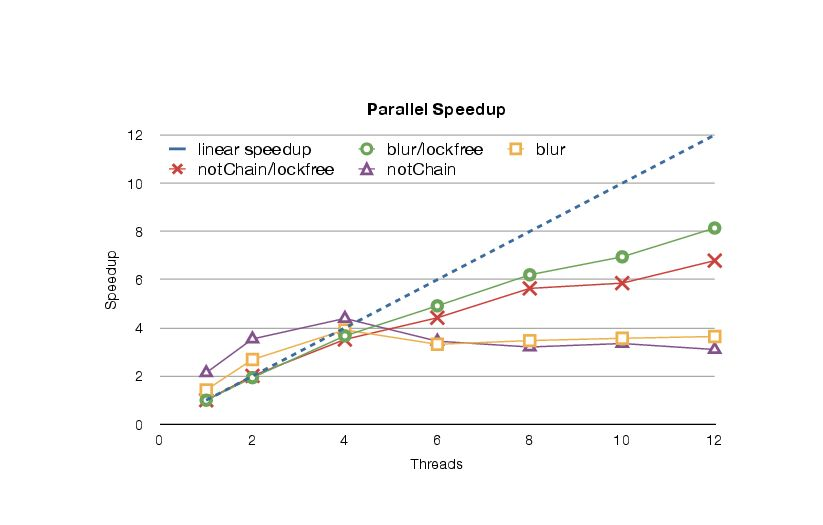
\includegraphics[width=1.0\columnwidth]{Figures/speedup.jpg}
}
\caption{Performance of LVish on parallelizing k-CFA\cite{lkuper2}}
\label{Figure2}
\end{figure}
setting\cite{newton2}. Distributed systems involve replication of data objects across several locations making them robust to data loss and provide better data locality. Eventual consistency is a policy where the updates for data objects \textbf{\textit{eventually}} reach the replicas, that need not always agree on queries. Convergent replicated data types provide a mathematical framework for reasoning about and enforcing the eventual consistency of such replicated objects, based on viewing them as elements of a lattice and replica conflict resolution as the lattice's join operation. CvRDTs are provably eventually consistent, but queries of CvRDTs allow inconsistent intermediate states of replicas to be observed. LVar-style threshold queries to CvRDTs extend them with support for deterministic queries and show that they are strongly consistent queries. A threshold query that returns an answer when executed on a replica will return the same answer every subsequent time, and on a different replica, it will eventually return the same answer, otherwise will block until it does so. It is therefore impossible to observe different results from the same threshold query, whether at different times on the same replica, or on different replicas.\par
\cite{newton1}discusses the viability of Lvish for certain graph algorithms, its drawbacks and enhancements. Lvish side effects are only monotonic updates. If a data structure needs to be updated multiple times, it will have to be done out of place by allocating LVars frequently, resulting in additional memory allocation and inefficiency relative to the in-place versions. Blocking $get$ semantics could slow down the performance until the dependency is met. Instead of blocking, the tasks could be retried at a later time/rescheduled when there dependency has been satisfied and the paper proposes an abort/retry feature for the same. The overhead in going through the scheduler many times has also been highlighted for applications like Maximum independent set.
\section{Summary}
\label{summary}
In an attempt towards creating better deterministic parallel programming models, Lvish has extended the existing theme of monotonicity to provide better applicability, usability, performance and a single generic model that subsumes many of the single assignment models, thereby representing a larger class of problems which can be efficiently parallelized. The performance with regards to certain benchmarks are an evidence of the same. At the end of the previous section, some of the drawbacks and a proposed enhancement were highlighted from a recent paper.
% Put citations from bibtex into References section which were not
% explicity cited.
\bibliographystyle{plain}
% Literature sources are to be found in seminarpaper.bib
\bibliography{seminarpaper} 
\end{document}
